\section{Three-Class Classification}
\lb{sec:3class}

One of the caveats of the analysis with two classes is that there are associated sources which do not belong to the AGN or PSR classes. 
These sources have the labels: unk, spp, glc, snr, gal, sbg, GAL, sfr, bin, SNR, HMB, LMB, css, PWN, pwn, hmb, SFR, BIN, lmb, NOV.
We collect all associated sources, which do not belong to AGN and PSR classes, into a new class, which we label as ``OTHER''.
Since in two-class classification we train algorithm to classify sources only into AGN and PSR classes, OTHER sources are also classified as either AGN or PSR.
This introduces a bias in the estimates of the number of AGNs and pulsars among unassociated sources.
One possibility to correct this bias is to assume that the fraction of OTHER sources among associated and unassociated sources are the same (Eq. (\ref{eq:other_correction})).
This correction can be applied for the total number of sources or for the number of sources in some window of parameters,
e.g., in a flux bin or in a range of latitudes and longitudes.
This is a straightforward calculation but it has some limitations. 
In particular, it implicitly assigns one probability for each AGN and one probability for each PSR to belong to the OTHER class inside a selected range of parameters.
For a small range of parameters the variance of this estimate can be very large due to a small number of associated OTHER sources in this parameter range.
As we will see in Section \ref{sec:pop_studies}, this correction depends on the choice of the variable used for binning, e.g.,
overall correction with latitude bins is not equal to the correction with longitude bins.

In this section we discuss the construction of probabilistic catalogs with multi-class classification (3-class classification in our case).
We start with the construction of the probabilistic catalog based on 3FGL by adding the class ``OTHER'', which includes all associated sources without AGN or PSR associations: there are 113 such sources in 3FGL (108 OTHER sources are without missing or unphysical values).
We use the same 11 features as in the 2-class classification: the only difference is that we use cos(GLON) instead of GLON.
The reason for this is that the LR and NN methods have a significantly worse performance than RF and BDT methods when we use GLON,
but, as we show below, all four methods have comparable accuracy when we use cos(GLON).
This may be due to a discontinuity in the GLON variable. 
We perform optimization of the meta-parameters for the four ML algorithms with the 3 classes.
In the calculation of accuracy we determine the probabilistic class as the class with the maximum probability among the three classes,
in some cases the maximal probability can be less than 0.5, but it is always above 1/3.


\begin{figure}[h]
\centering
%\hspace*{-1cm}
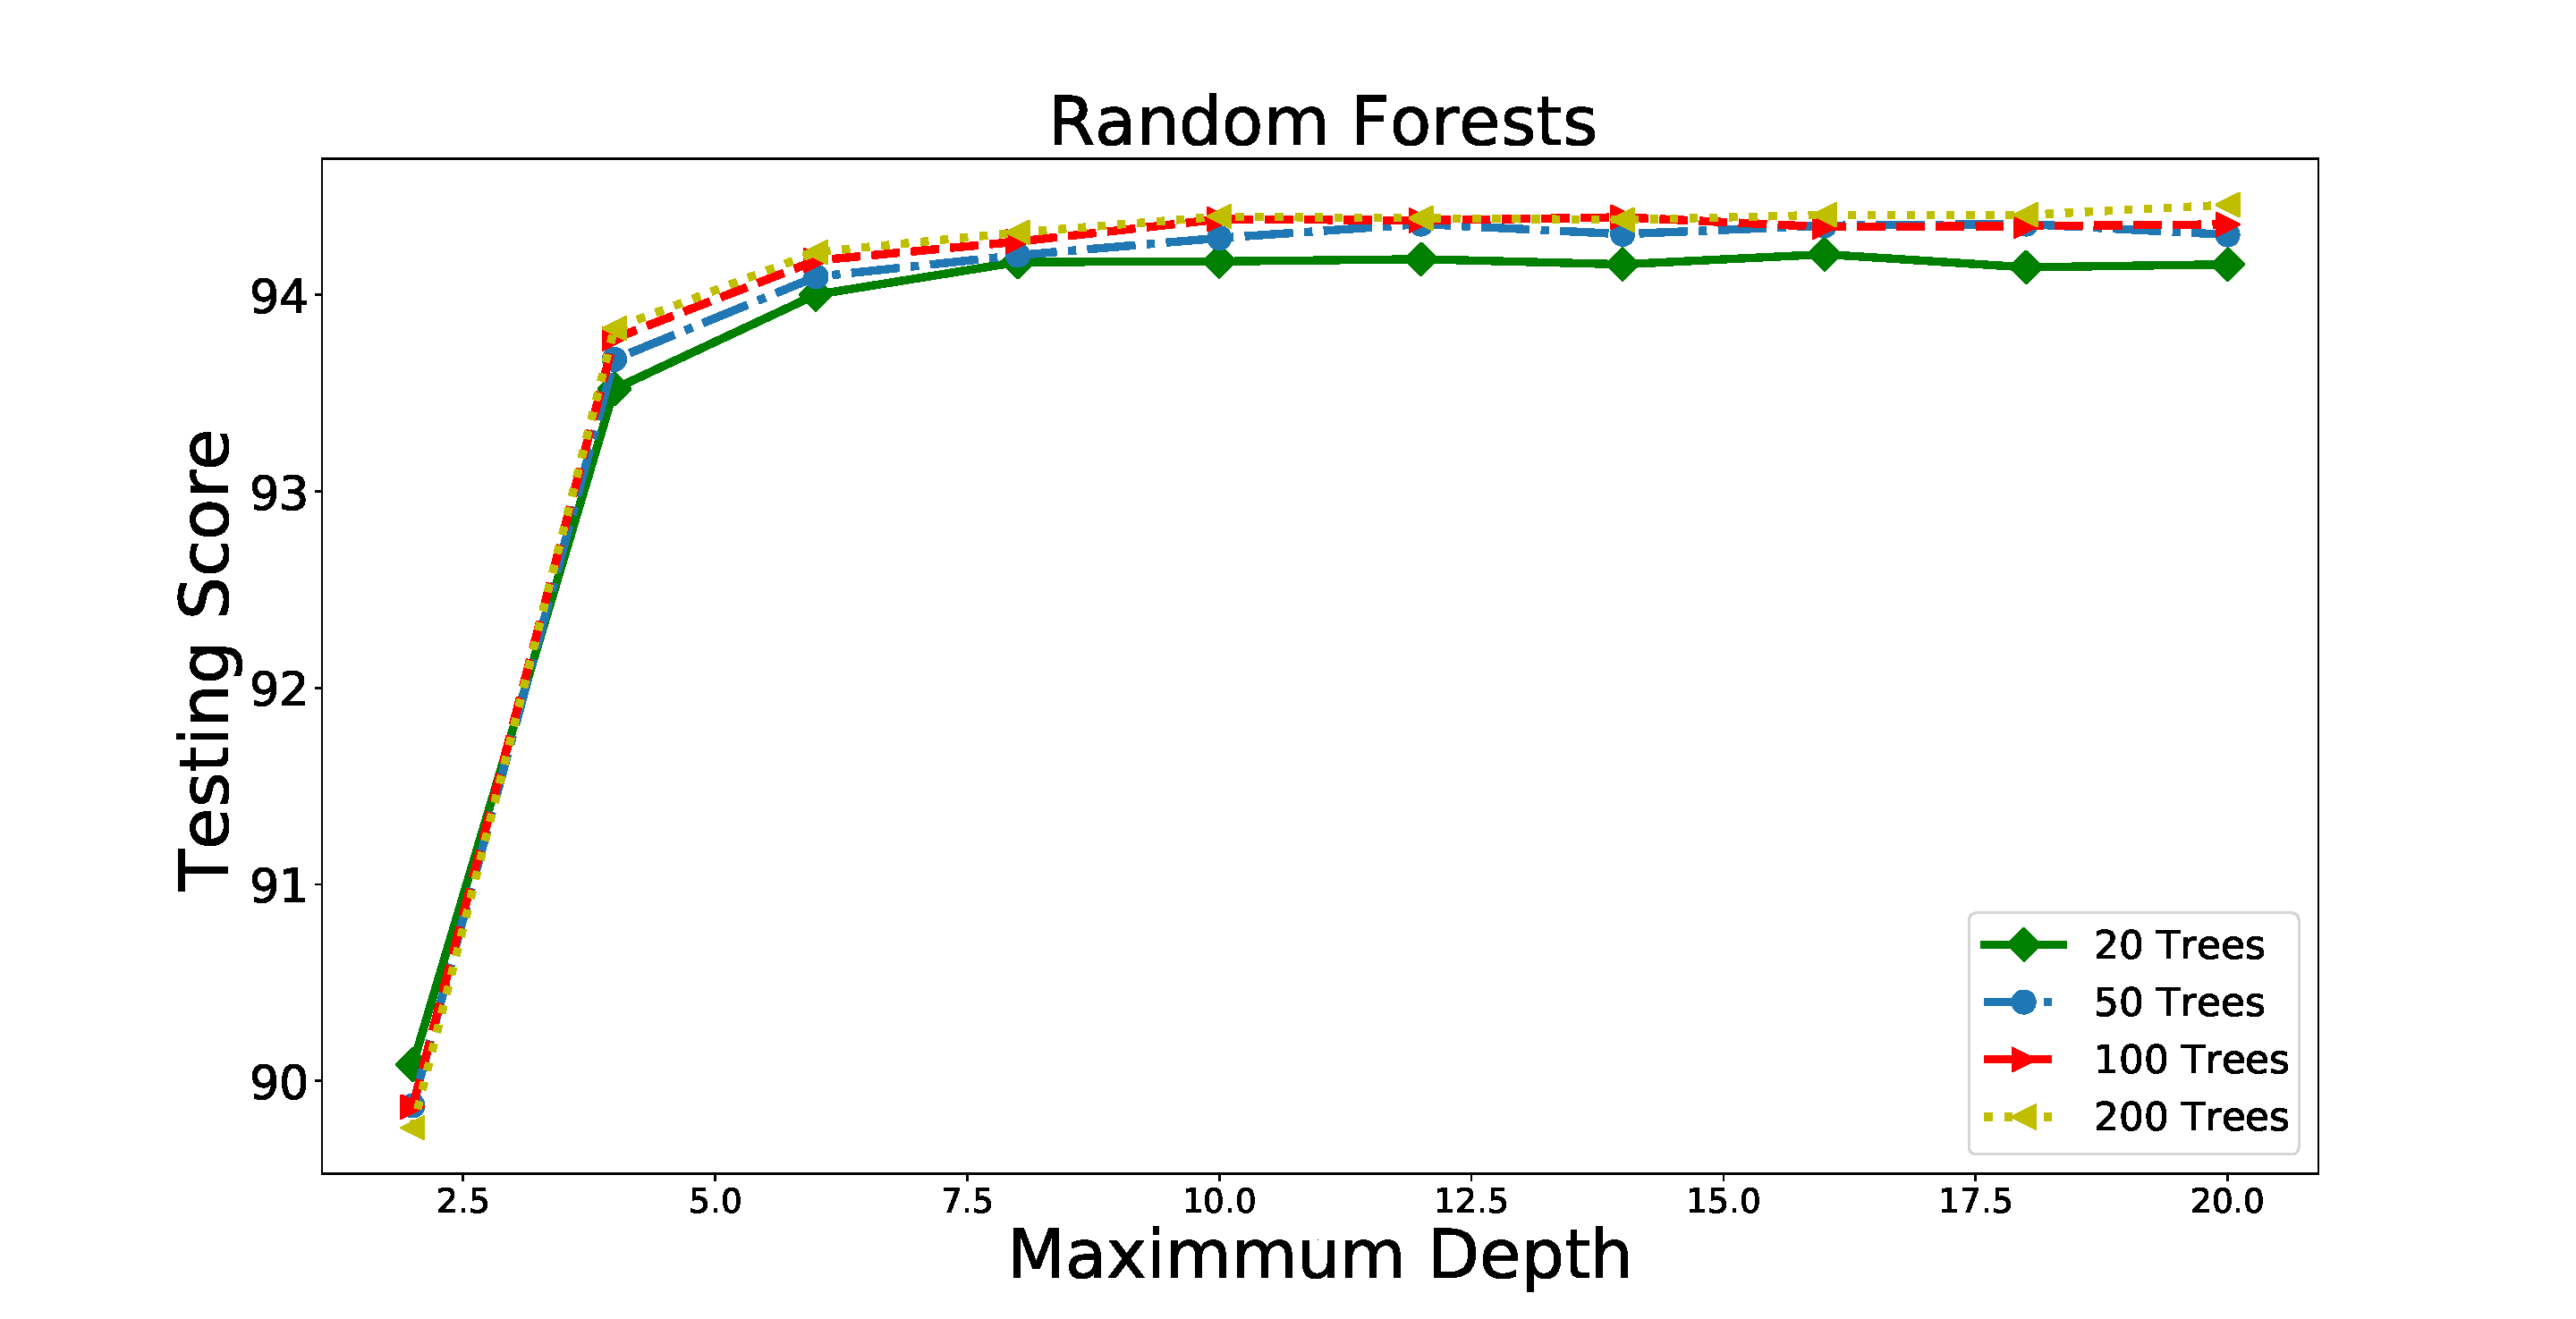
\includegraphics[width=0.5\textwidth]{plots/rf_train_multi.pdf}\\
%\hspace*{-1cm}
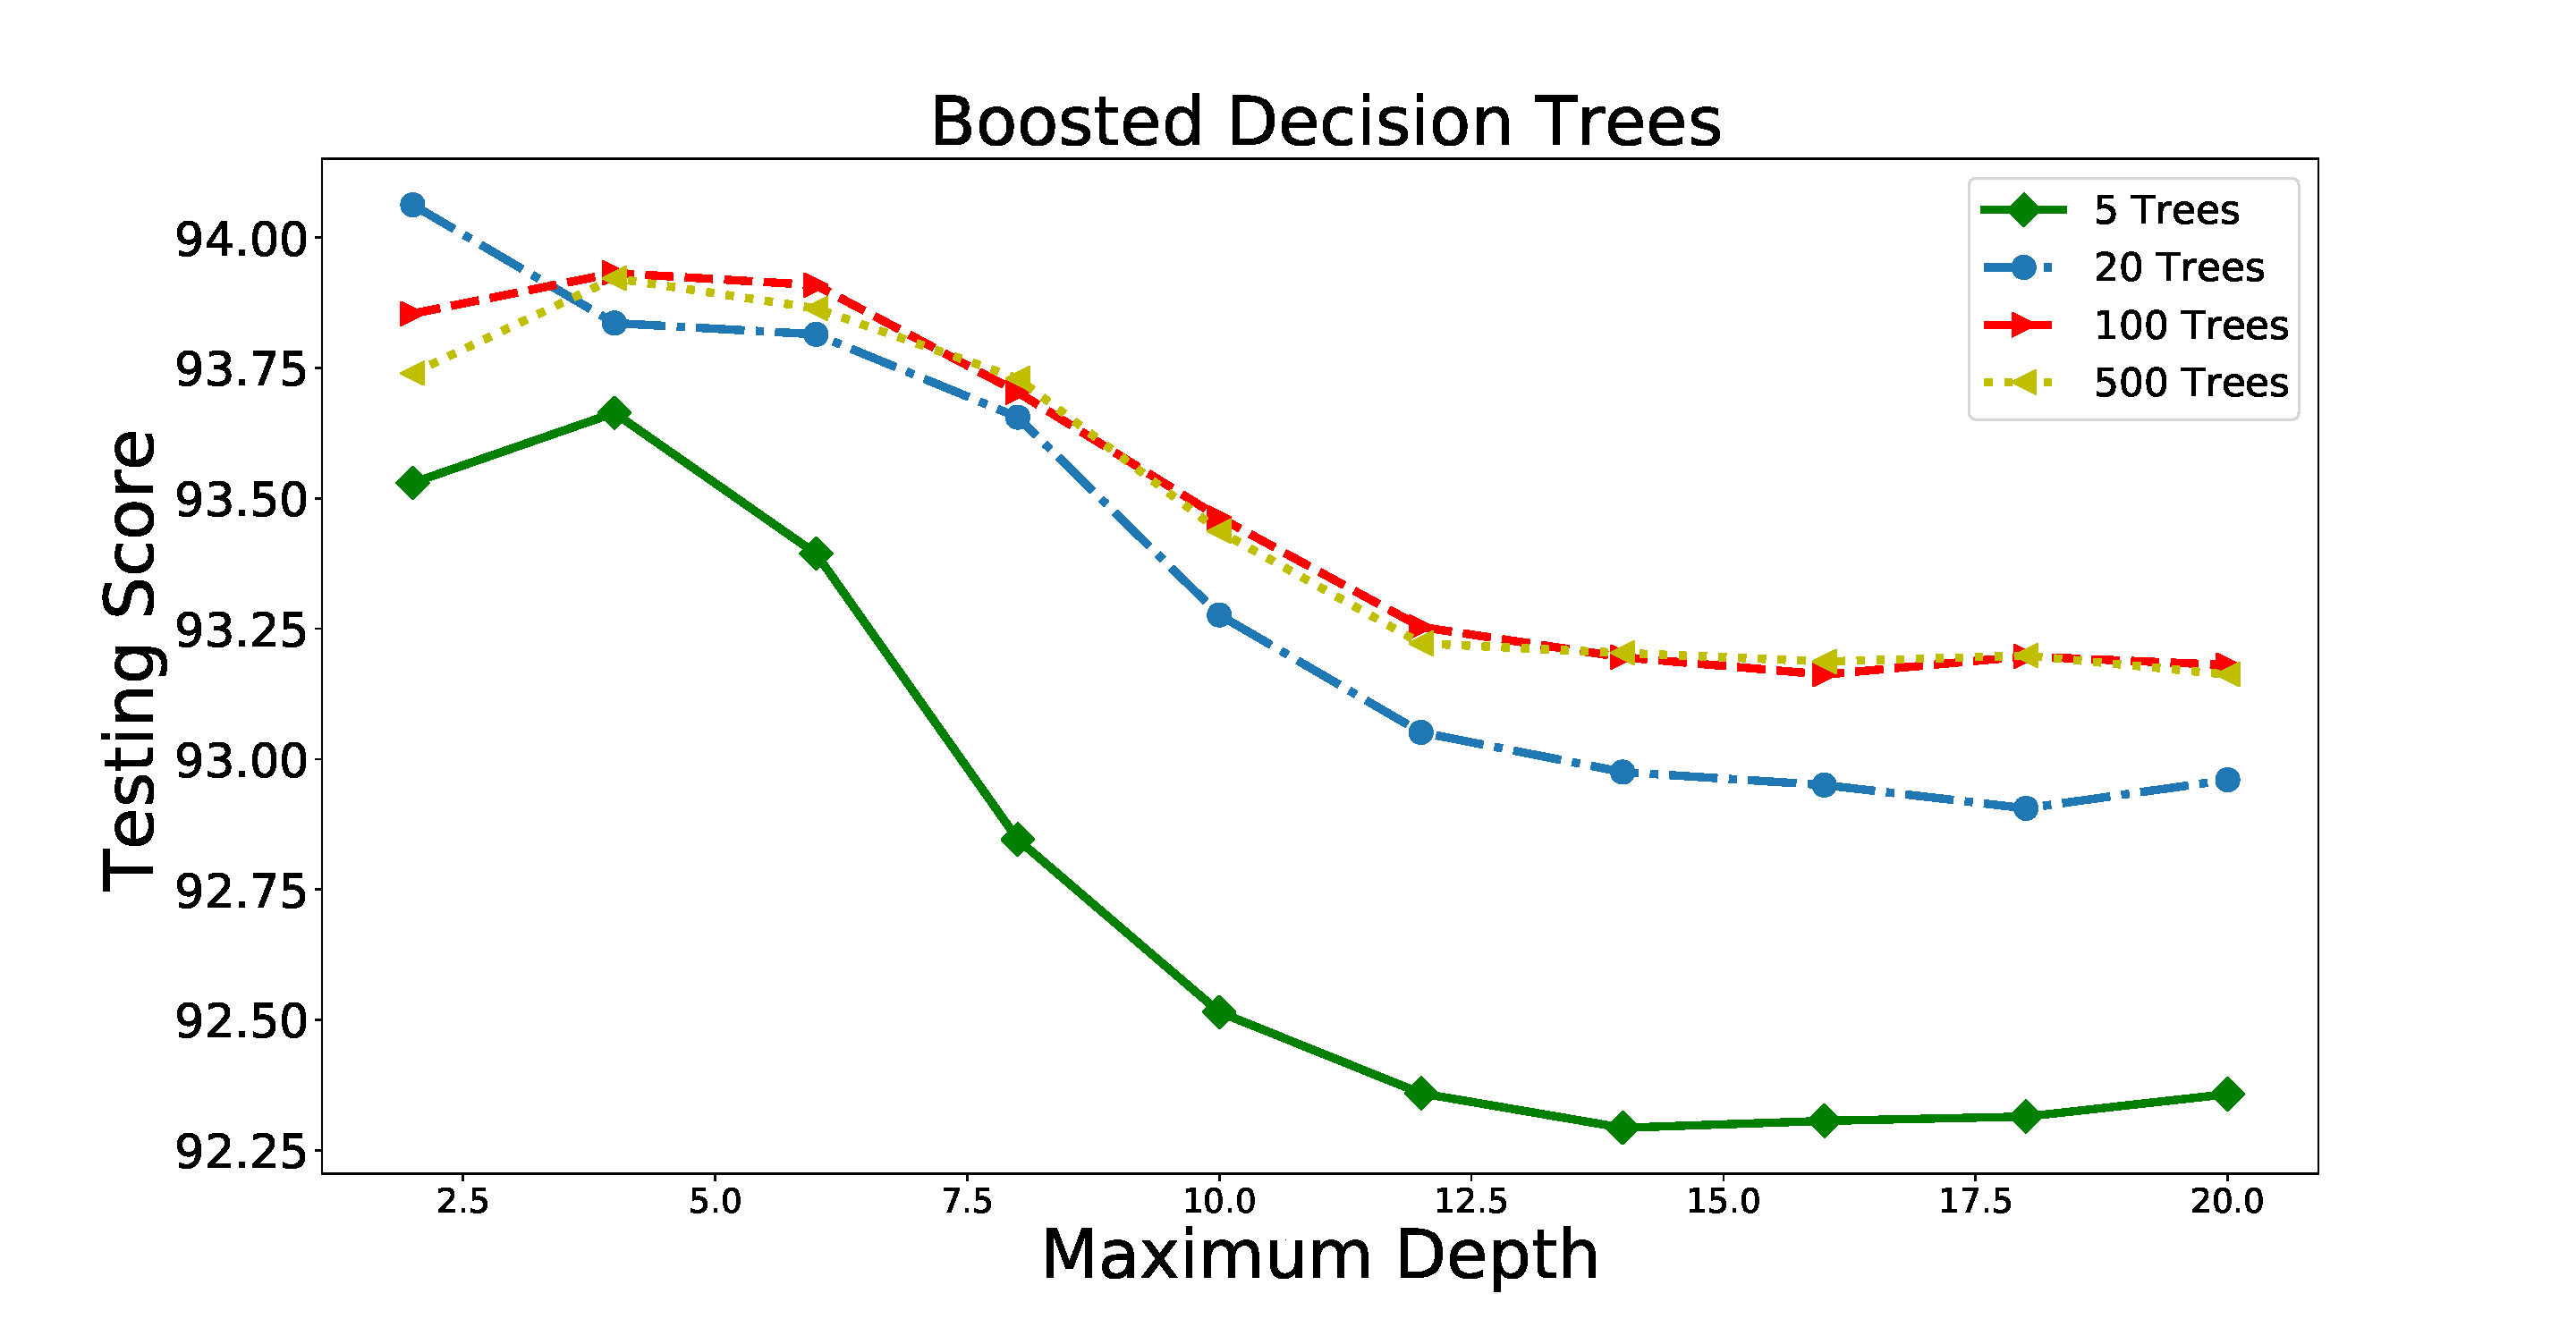
\includegraphics[width=0.5\textwidth]{plots/bdt_train_multi.pdf}
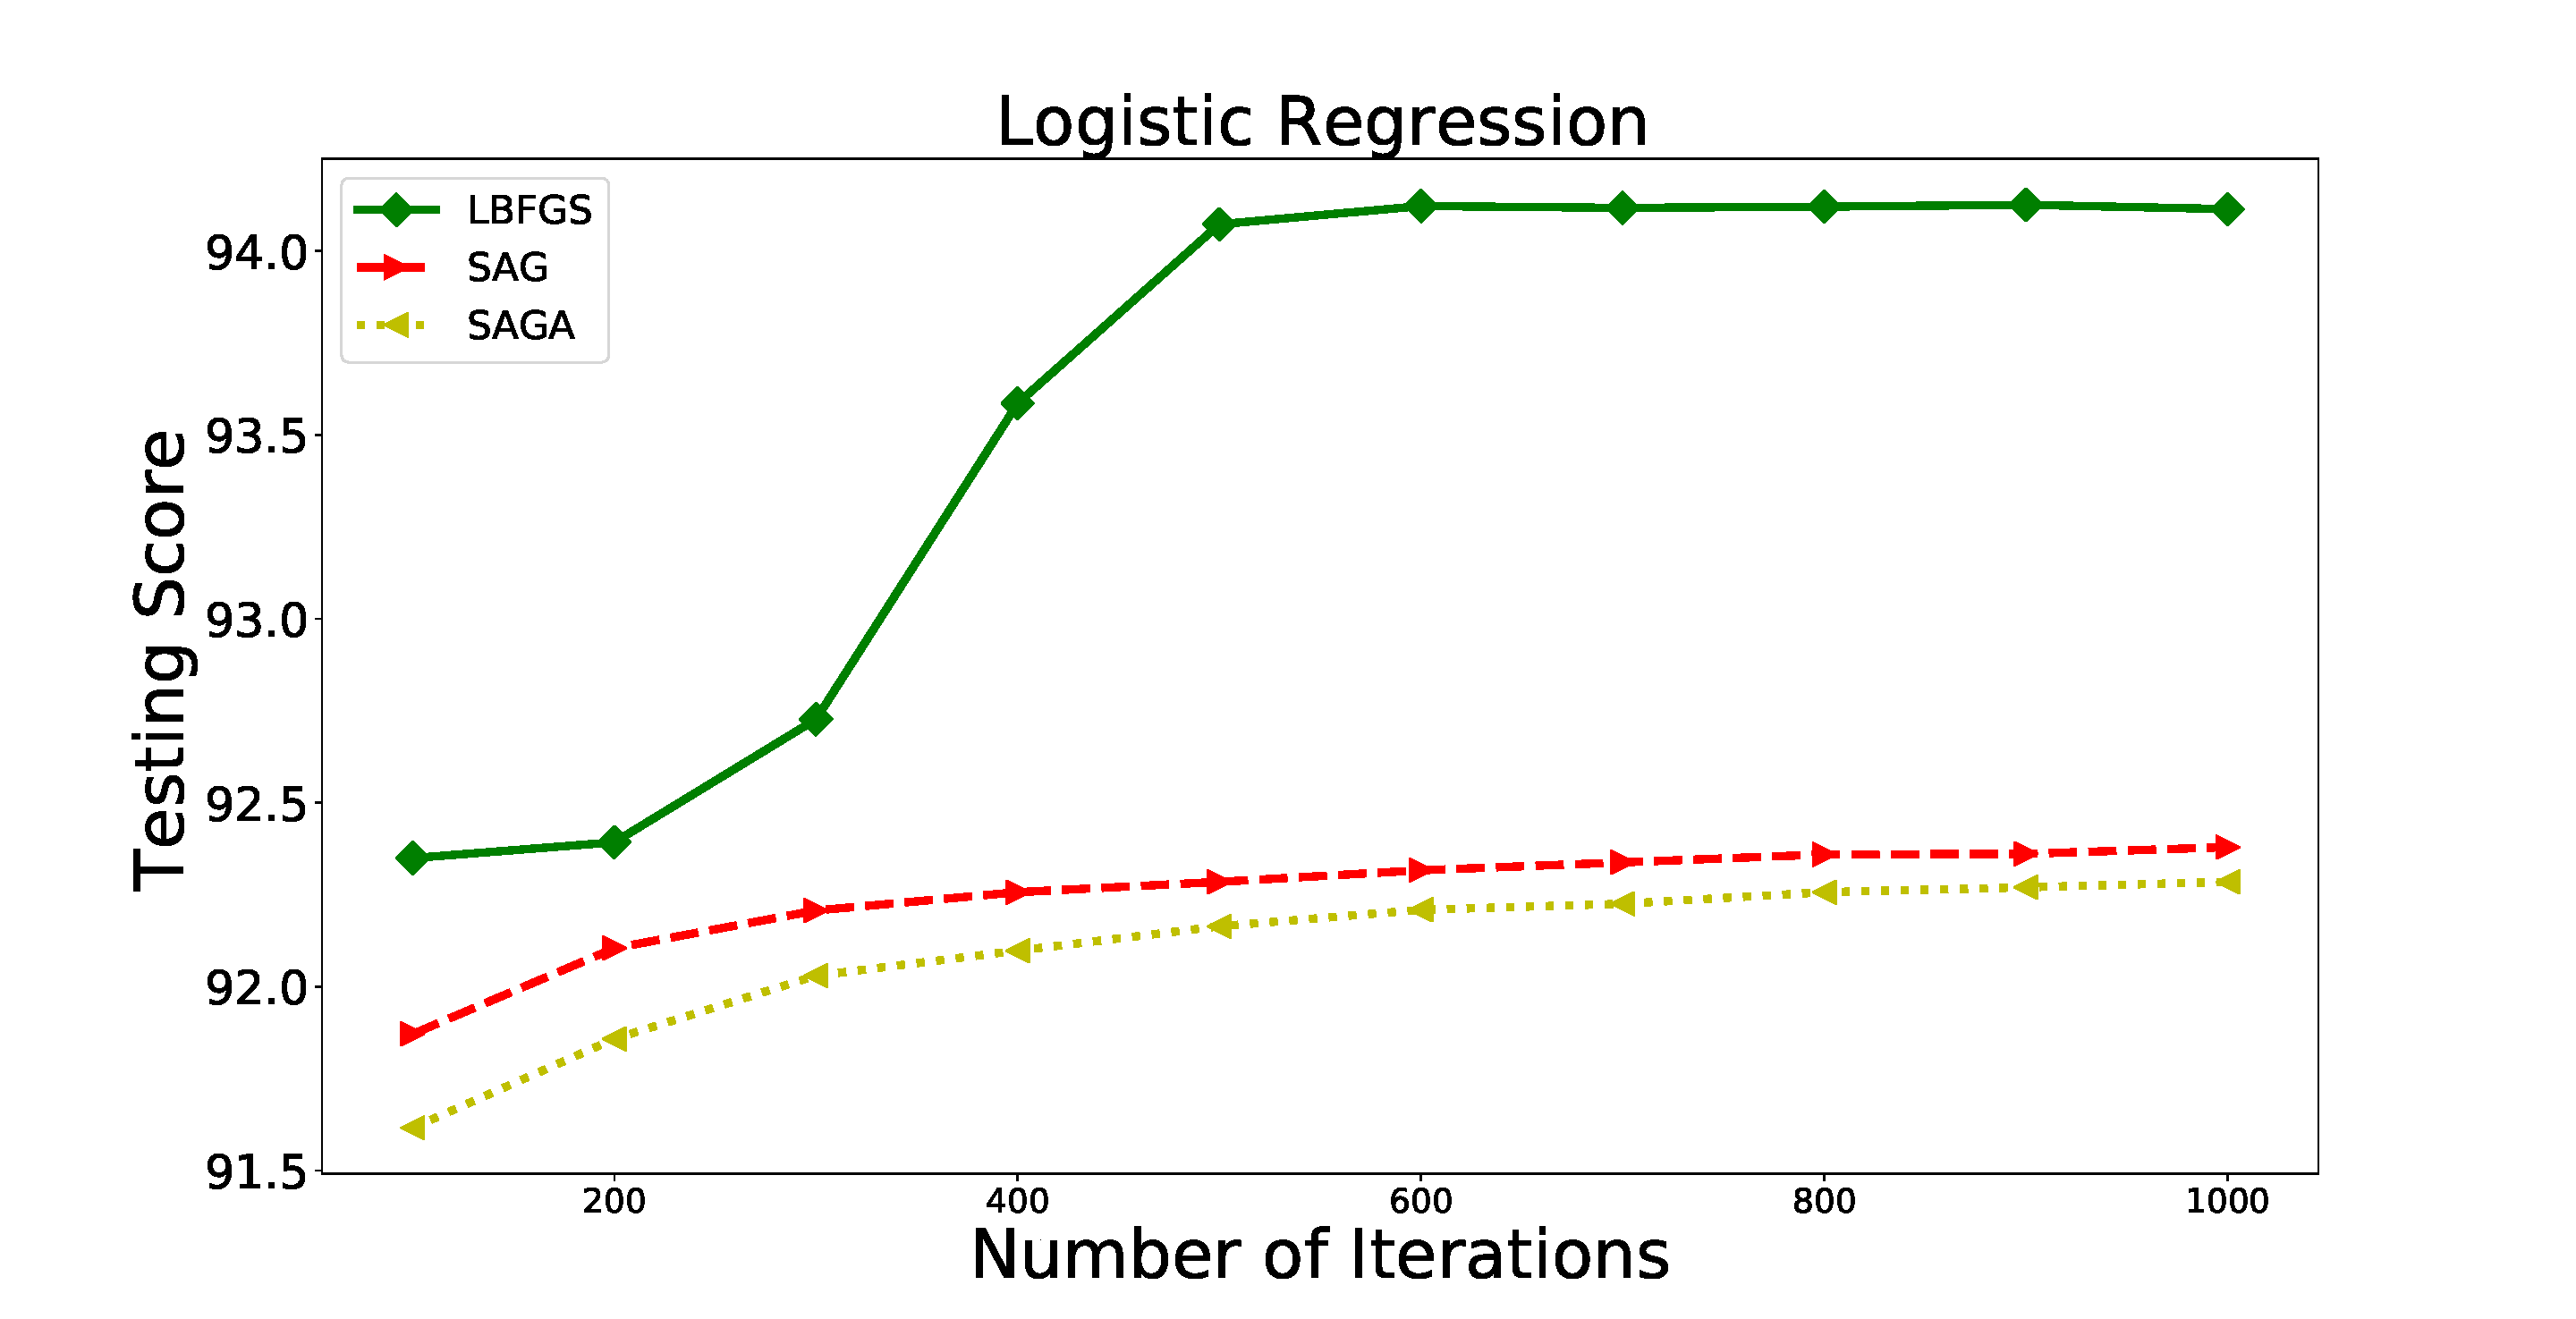
\includegraphics[width=0.5\textwidth]{plots/lr_train_multi.pdf}
\caption{Accuracy of the 3-class classification with RF, BDT and LR  methods. LR does not have liblinear solver here, since liblinear 
does not support multi-class loss.
}
\label{fig:tree_multi}
\end{figure}

\begin{figure}[h]
\centering
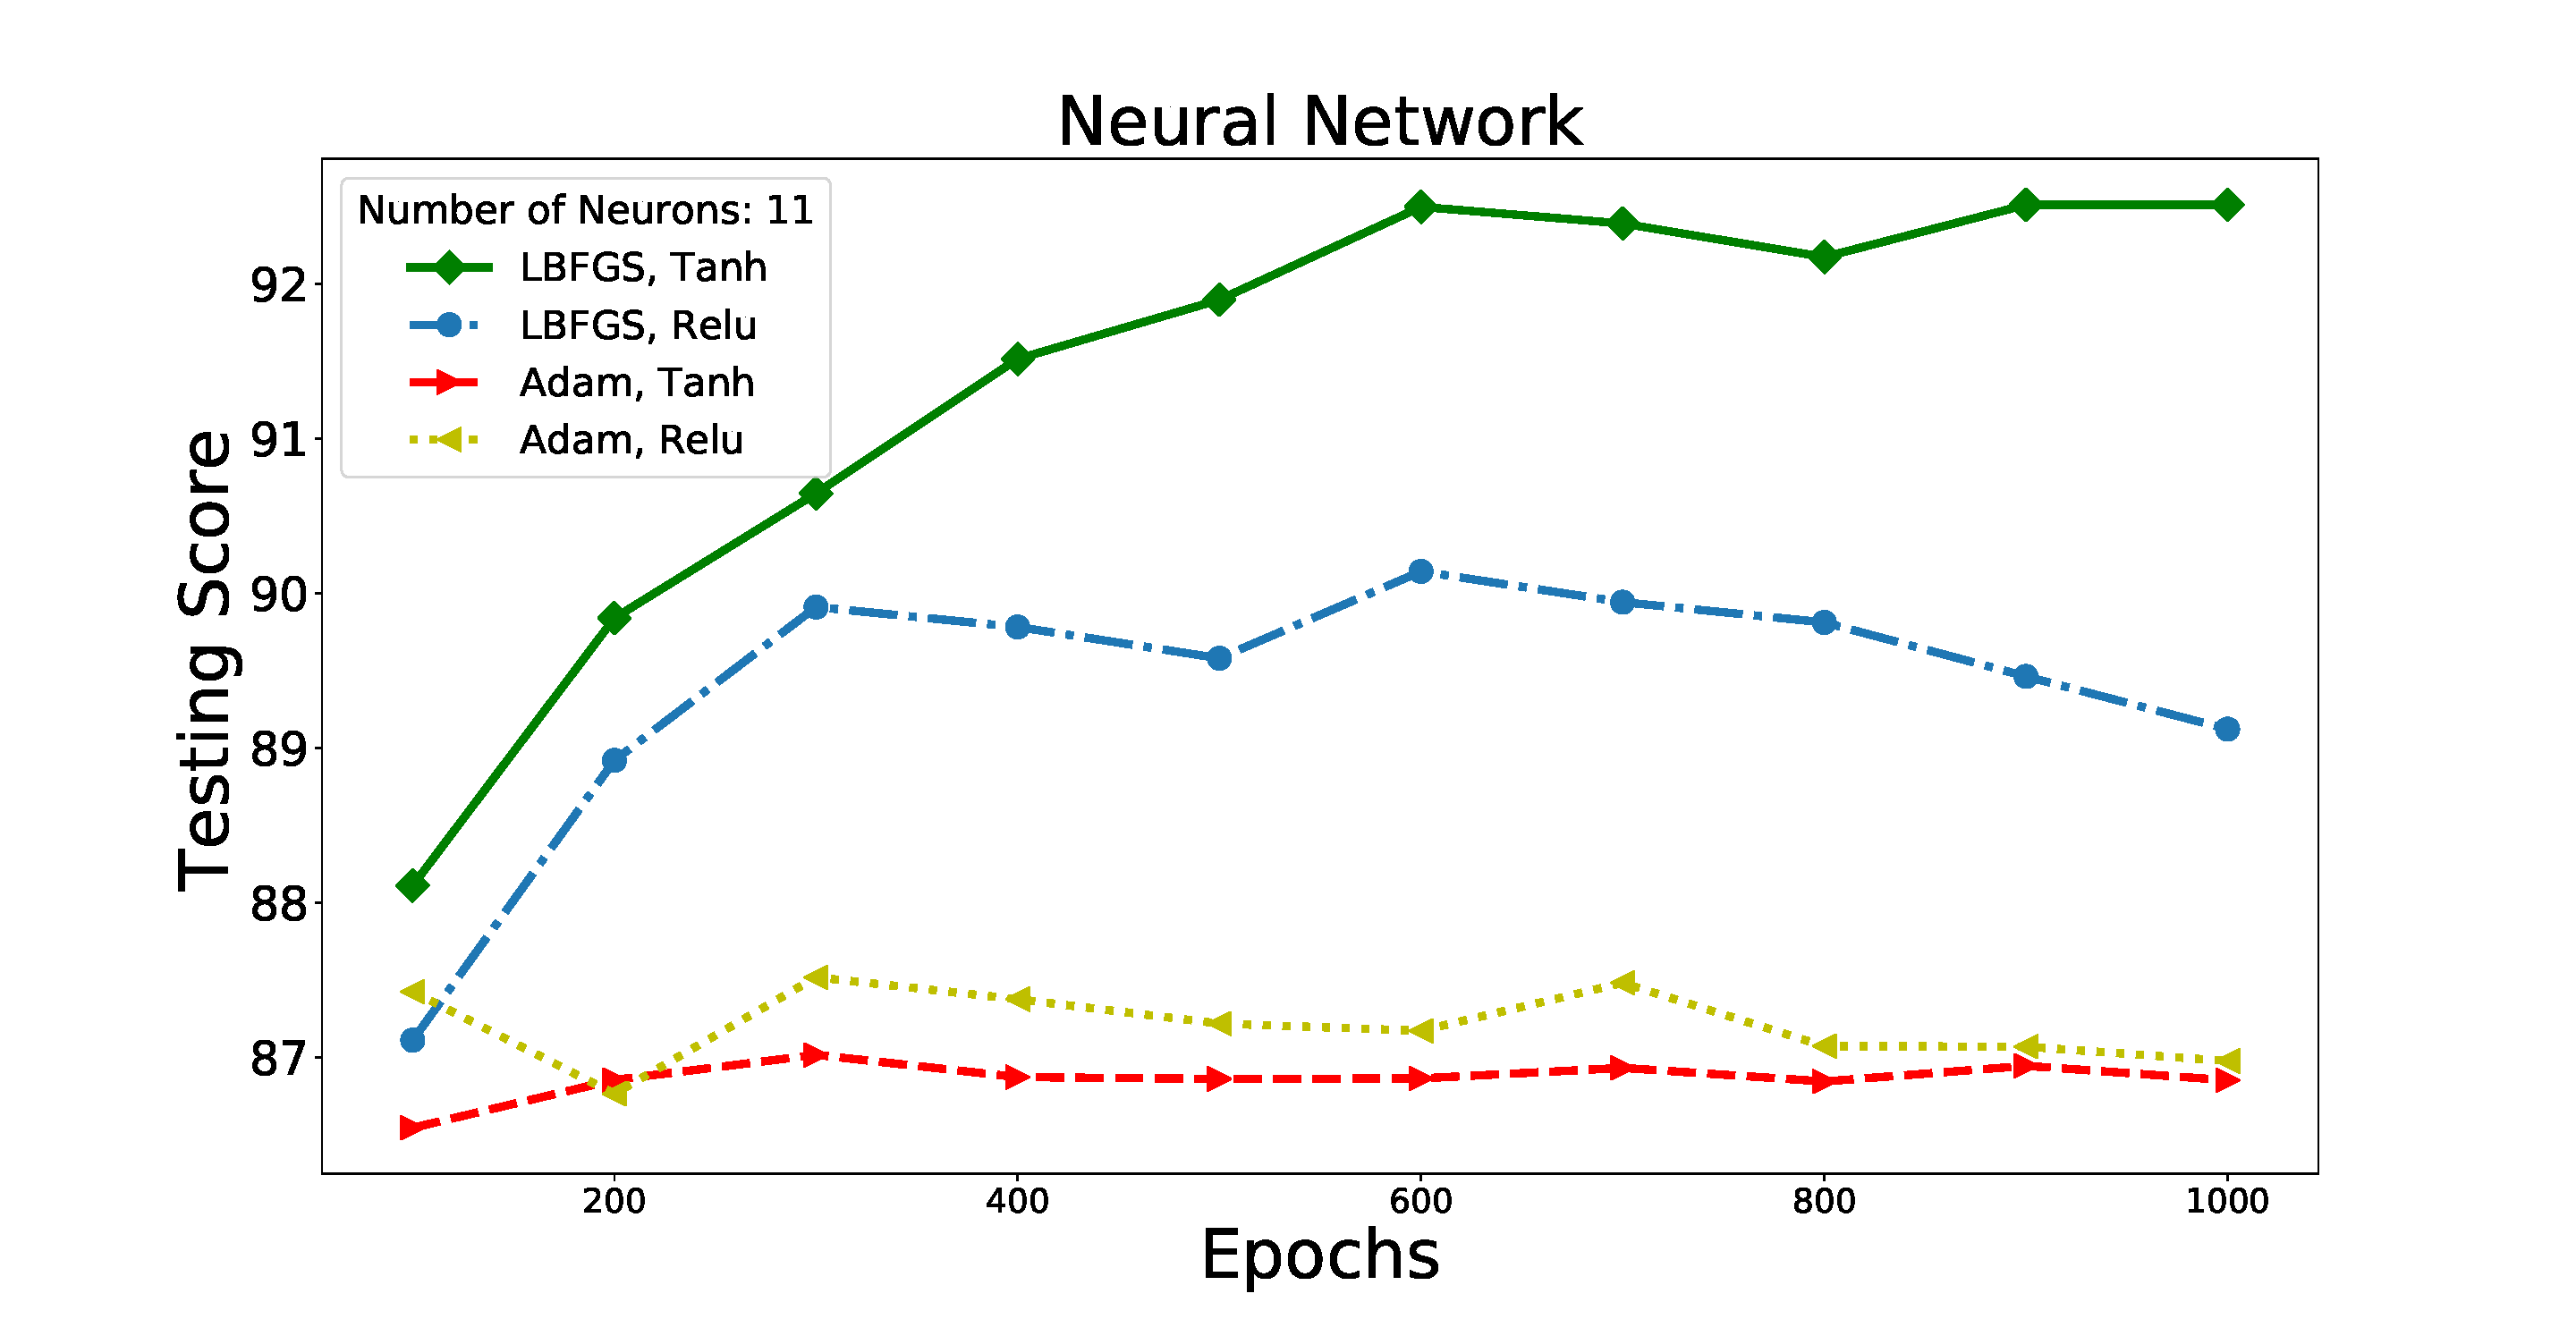
\includegraphics[width=0.5\textwidth]{plots/nn_epoch_train_multi.pdf}\\
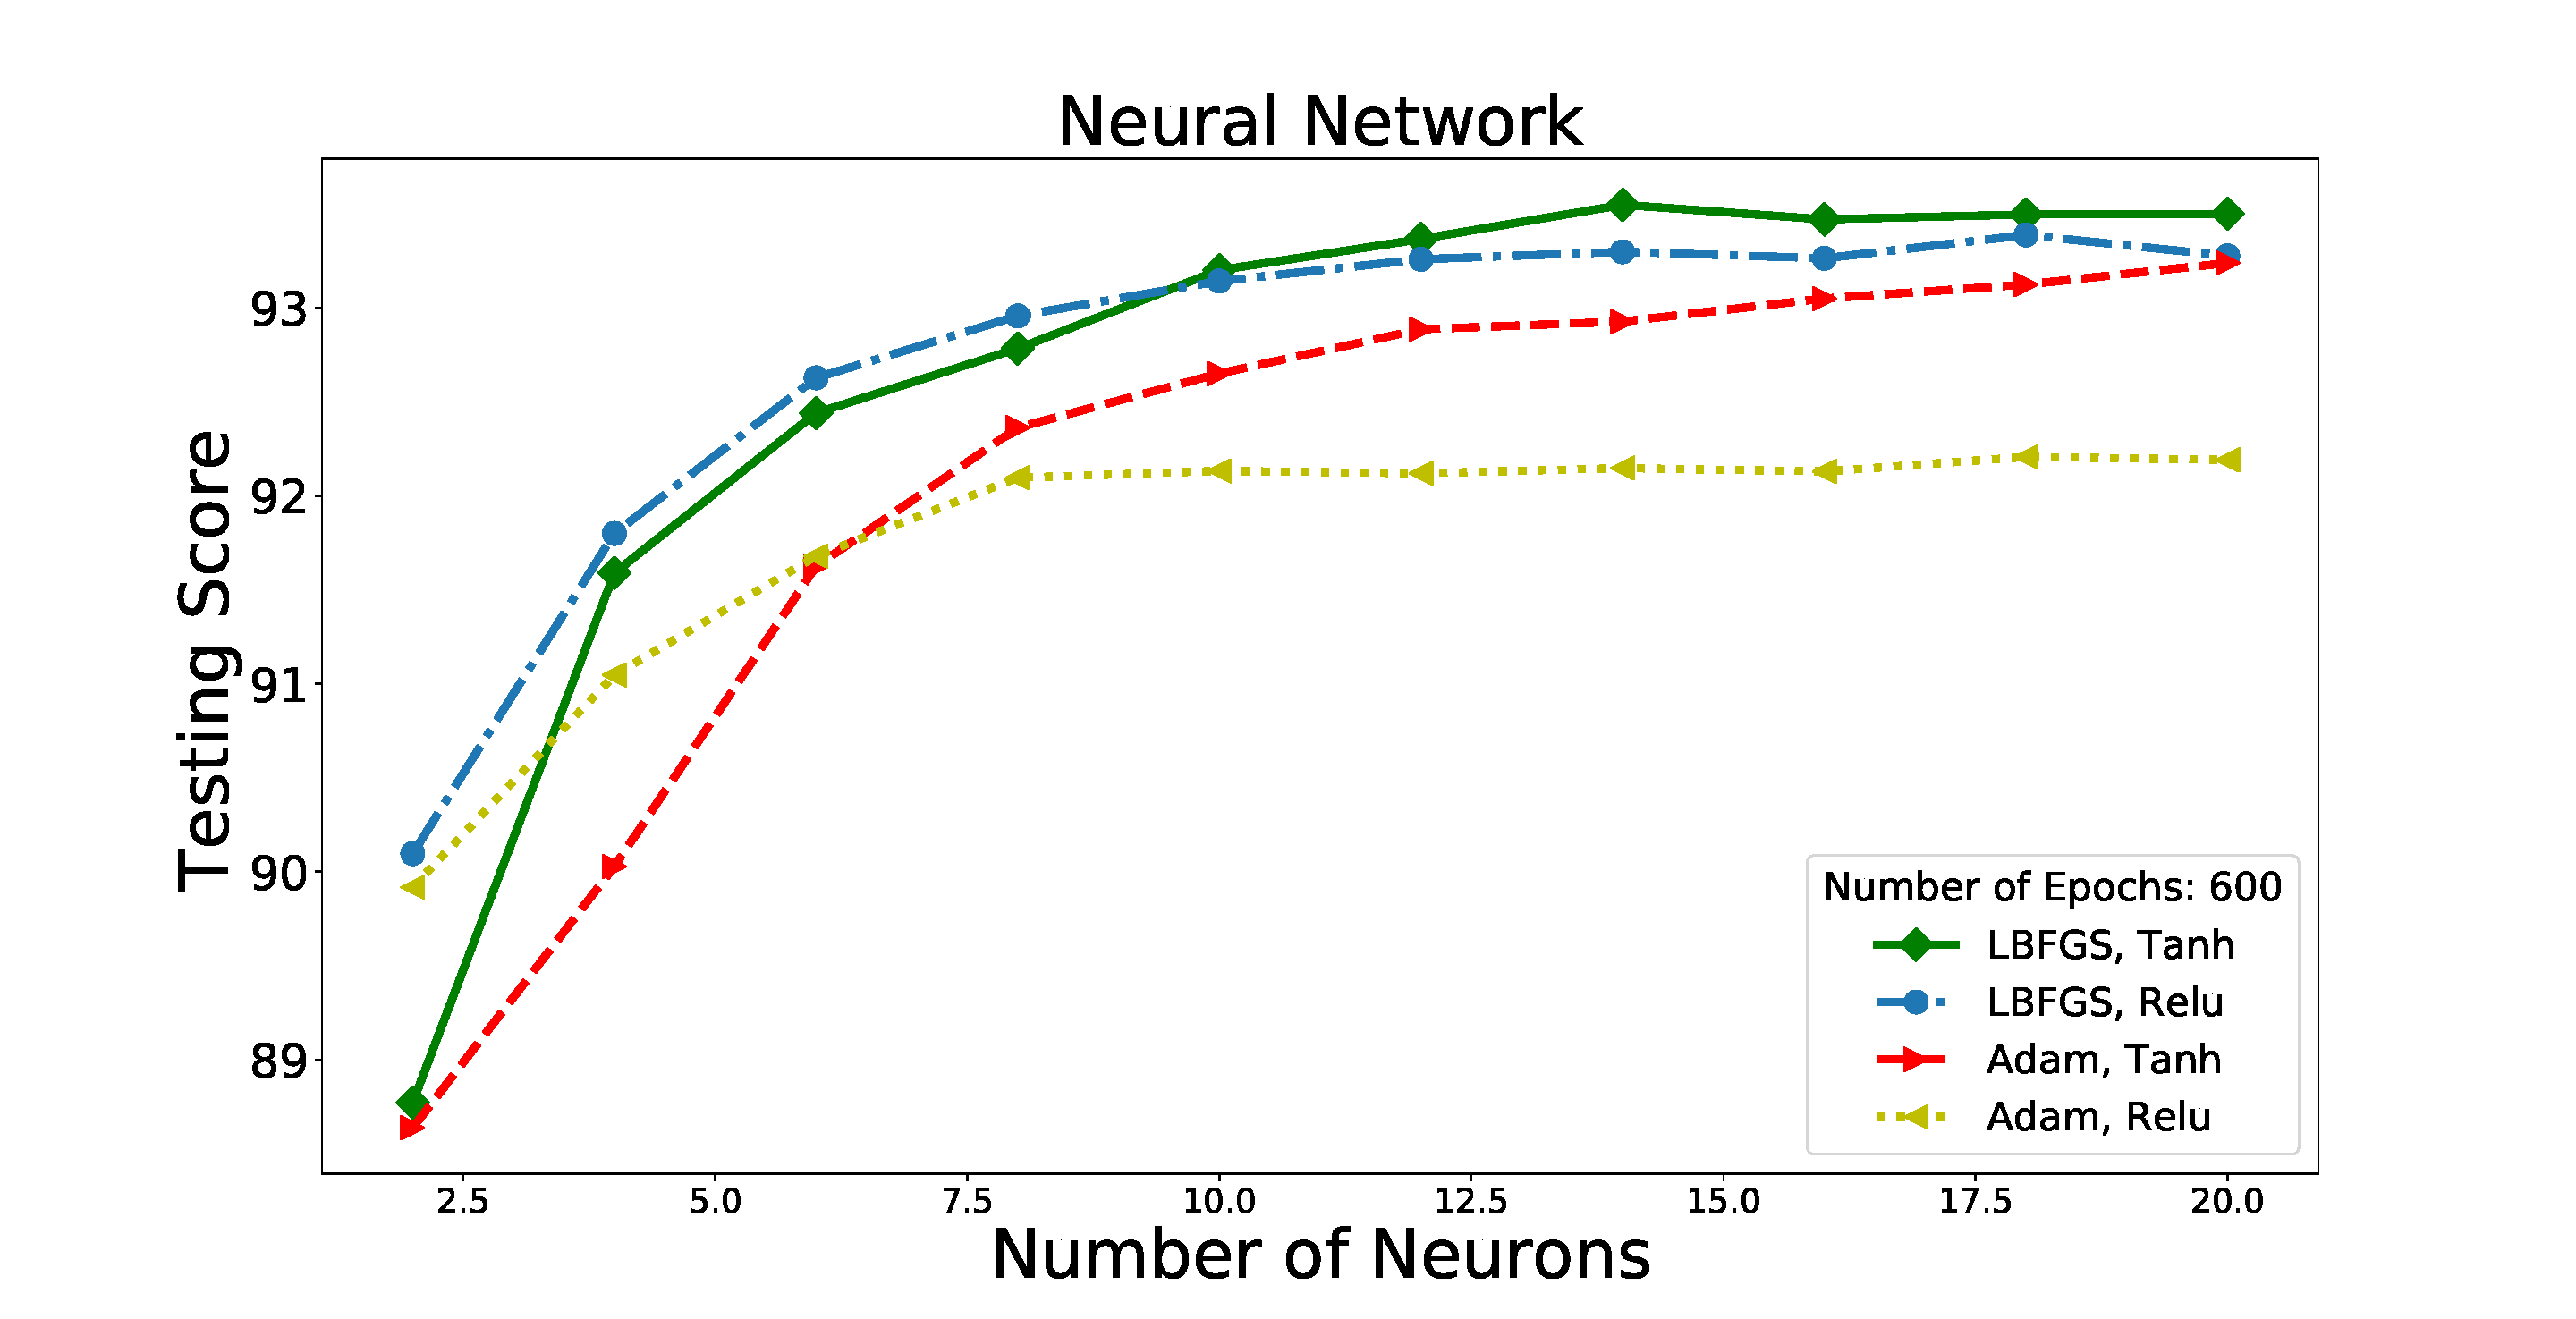
\includegraphics[width=0.5\textwidth]{plots/nn_neuron_train_multi.pdf}
\caption{Accuracy of the NN classification as a function of the number of epochs and of the number of neurons
 for the 3-class classification. 
 }
\label{fig:nets_multi}
\end{figure}


The dependence of accuracy on meta-parameters of the algorithms is shown in Figs. \ref{fig:tree_multi} and \ref{fig:nets_multi}.
We see that for the tree-based algorithms, the optimal parameters are similar to the 2-class classification, i.e., 50 trees with depth 6 for RF and 100 trees with depth 2 for BDT 
provide close to optimal performance at a minimal cost in complexity (depth of the trees).
The main difference for NN and LR algorithms is that more steps are needed for convergence, especially in the case of oversampling. 
In the following we use 600 epochs for NN and 500 iterations for LR instead of 300 epochs and 200 iterations respectively in the two-class case.
For NN, the accuracy stops increasing above about 10 neurons in the hidden layer (in the following we use 11 neurons for classification: the same as in the two-class case).
For oversampling, we use the oversampling factors $\sqrt{\frac{\text{\# AGN}}{\text{\# PSR}}}$ and $\sqrt{\frac{\text{\# AGN}}{\text{\# OTHER}}}$ for PSR and OTHER classes respectively (compared to the $\frac{\text{\# AGN}}{\text{\# PSR}}$ oversampling factor in the 2-class case).
The reason for the smaller oversampling factors is to avoid overweighting the two relatively small PSR and OTHER classes.

\begin{figure}[h]
\centering
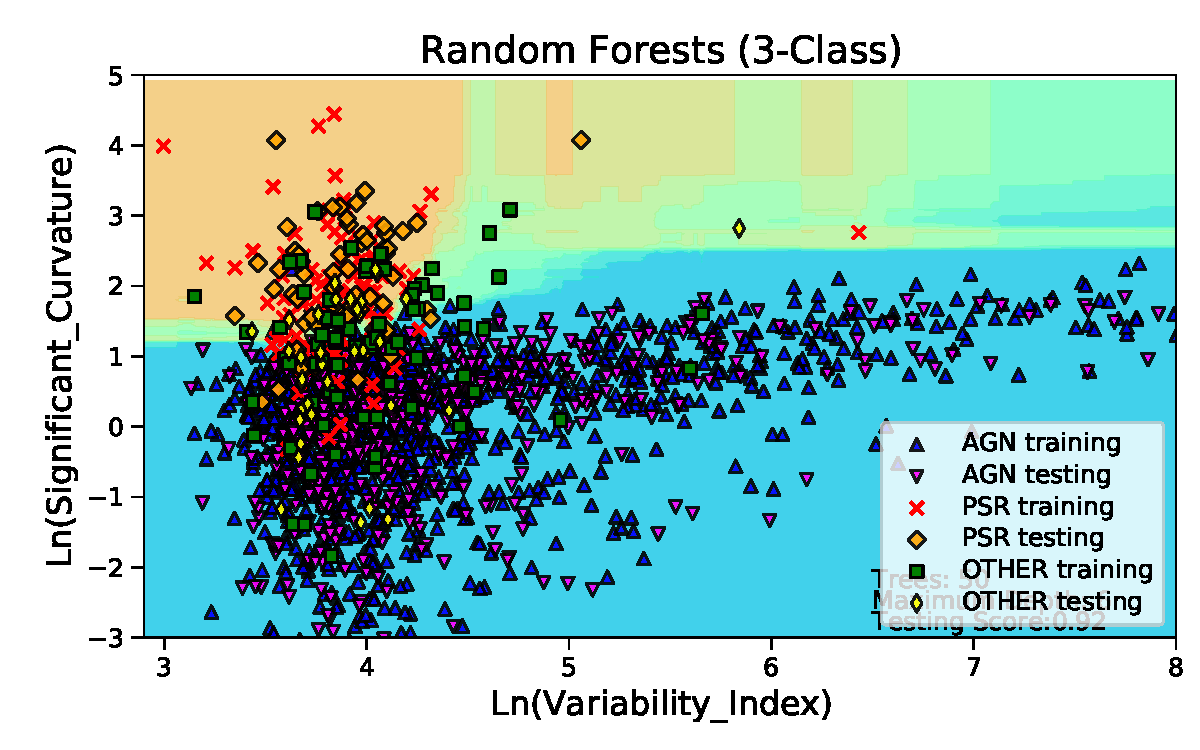
\includegraphics[width=0.46\textwidth]{plots/classification_domains/rf_50_6_3class.pdf}
\caption{Classification domains for RF in the 3-class classification.
The sources in the blue, green, and brown areas are attributed to AGN, OTHER, and PSR classes respectively.
}
\label{fig:RF_domains_3class}
\end{figure}

We show an example of domains in the 3-class case in Fig. \ref{fig:RF_domains_3class}.
A class domain is determined by the class with the largest probability.
Since in the 3-class case there are two independent probabilities, which are difficult to show with a single color bar,
we present only the domains represented by three different colors: brown for PSR, green for OTHER, and blue for AGN classes.
The corresponding training and testing data are shown by red crosses and brown rotated squares for PSR, by green squares and yellow diamonds for OTHER,
and by blue and purple triangles for AGN.
The classification domains are averaged over 100 realizations of splitting the data into training and testing samples.
One of these splittings is shown in the figure for illustration.


The accuracies of our chosen models for classification of the 3FGL sources are presented in Table \ref{tab:selected_algs_multi}.
As in the 2-class case, the accuracies are averaged over 1000 realizations of splitting the data into training and testing samples.
We notice that accuracies presented in Table \ref{tab:selected_algs} are calculated relative to AGN and PSR classes only. If we take into account that all OTHER sources
are misclassified in this case, then the testing accuracy is reduced by about 5\% (the fraction of OTHER sources among associated sources in 3FGL),
while the accuracy of comparison with 4FGL-DR2 is reduced by about 10\% (there are 37 unassociated sources in 3FGL with OTHER class associations in 4FGL-DR2,
while there are in total 340 unassociated sources in 3FGL with associations in 4FGL-DR2).
Thus the testing accuracy of 93-94\% in Table \ref{tab:selected_algs_multi} provides at least a 1-2\% improvement over the accuracy in Table \ref{tab:selected_algs},
after taking into account the misclassification of OTHER sources in the 2-class case.
A similar improvement is seen for the accuracy of classification of unassociated sources in 3FGL with corresponding 4FGL-DR2 associations.

Similarly to the 2-class classification, we use the condition that all algorithms agree to determine the candidate probabilistic classes of sources.
In the end of this Section we also use a stricter condition that the sum of probabilities is larger than 7 in order to determine lists of most likely PSR and OTHER source candidates.
A comparison of predicted classes (using the all algorithms agreement condition) for the 3FGL unassociated sources in the 3-class classification case with the classes of the corresponding associated sources in the 4FGL-DR2 catalog are presented in Table~\ref{tab:3FGL_vs_4FGL_3class}.
It is interesting to note that there are fewer sources with mixed classification in this case relative to the 2-class classification in 
Table~\ref{tab:3FGL_vs_4FGL_2class}.
Also the number of correct predictions in the 3-class case is 263 (out of 340 sources), while in the 2-class case there are 246 correct predictions.
We also show in this table the expected precision and recall for the all-algorithms-agree and $\sum_a p_a > 7$
conditions.
We note that in spite of adding an additional class, the precision of the AGN and PSR classifications in 3FGL
is higher in the 3-class case (Table~\ref{tab:3FGL_vs_4FGL_3class}) compared to the 2-class case
(Table~\ref{tab:3FGL_vs_4FGL_2class}), but the recall is smaller for pulsars and similar or larger for AGNs in the 3-class case.

\begin{table}[!h]
    \caption{Testing accuracy of the selected algorithms for the 3-class classification of 3FGL sources.}
    \label{tab:selected_algs_multi}

\centering
\hspace{-0.2cm}
\resizebox{0.47\textwidth}{!}{
    \tiny
  \centering
    \renewcommand{\tabcolsep}{0.4mm}
\renewcommand{\arraystretch}{1.6}

%\hspace{-3mm}
    \begin{tabular}{c c c c c c c}
    \hline
    \hline
    Algorithm&Parameters &  Testing\ &Std. Dev.& Comparison with \\
    & & Accuracy\ & & 4FGL-DR2 Accuracy \\
    \hline
    RF & 50 trees, max depth 6  & 93.96 & 0.85 & 85.00 \\
    RF\_O &   & 94.38 & 0.76 & 85.00 \\ 
    \hline
    BDT & 100 trees, max depth 2    &   93.72 & 0.83 & 83.24 \\
    BDT\_O &     &   93.83 & 0.80 & 85.29 \\
    \hline
    NN & 600 epochs, 11 neurons, LBFGS & 93.17 & 1.05 & 83.53 \\
    NN\_O &&  92.51 & 1.34 & 81.76 \\
    \hline
    LR & 500 iterations, LBFGS solver & 93.93 & 0.88 & 83.24 \\
    LR\_O &   & 93.01 & 0.96 & 83.24 \\
    \hline
    \end{tabular}}
    %\vspace{2mm}
    \tablefoot{
    Comparison with associations in the 4FGL-DR2 catalog
    is presented in the last column.
    ``\_O'' denotes training with oversampling.}
\end{table}


\begin{table}[!h]
    \caption{
    Comparison of classes predicted for unassociated sources in the 3FGL catalog using 3-class classification
    with associations in the 4FGL-DR2 catalog.}
    \label{tab:3FGL_vs_4FGL_3class}

\centering
\resizebox{0.45\textwidth}{!}{
    \tiny
 \renewcommand{\tabcolsep}{0.3mm}
\renewcommand{\arraystretch}{1.5}

    \begin{tabular}{l c c c c c c c}
    \hline
    \hline
    4FGL-DR2 class & \multicolumn{4}{c}{3FGL prediction} & Recall\ \ & Recall & Recall \\
      &\ AGN &\ PSR &\ OTHER &\ MIXED & (4FGL assoc) & (all agree) & ($\sum_a p_a > 7$)\\
    \hline
    AGN & 238 & 2 &  1 & 17 & 0.92 & 0.97 & 0.91\\ % 258
    PSR & 12 & 17 &  0 & 16 & 0.38 & 0.58 & 0.28 \\ % 45
    OTHER & 6 & 5 & 8 & 18 & 0.22 & 0.29 & --\\ % 37
    \hline
    Precision (4FGL assoc) & 0.93 & 0.71 & 0.89  \\
    Precision (all agree) & 0.99 & 0.89 & 0.75  \\
    Precision ($\sum_a p_a > 7$) & 0.99 & 0.98 & --  \\
    \hline
    \end{tabular}}
    %\vspace{2mm}
    \tablefoot{For the definition of precision and recall labels see Table \ref{tab:3FGL_vs_4FGL_2class}.}
\end{table}



The 3-class classification of 4FGL-DR2 sources is performed analogously to the 3-class classification of the 3FGL sources.
The differences between the 4FGL-DR2 and 3FGL 3-class classifications are similar to the differences in the 2-class classification of 3FGL and 4FGL-DR2 sources:
we use 16 features instead of 11 features in the 3FGL case (the features are the same as in the 2-class classification of 4FGL-DR2 sources in Section \ref{sec:4FGLprediction} but with GLON replaced by cos(GLON))
and we have 16 neurons in the hidden layer of the NN method. Furthermore, for LR we use 1000 iterations as it gives better performance for oversampled cases.
The corresponding accuracies are reported in Table \ref{tab:selected_algs_4fgl_multi}.
In comparing the accuracies with the 2-class classification in Table \ref{tab:selected_algs2}, 
one has to take into account that there are 346 OTHER sources among 4116 associated sources in 4FGL-DR2, which is about 8.4\%.
Since all OTHER sources are ``misclassified'' by the 2-class classification, the 3-class classification provides an improvement of about 2-4\% compared to the 2-class classification.

The expected precision and recall for the classification of sources using agreement among all algorithms and the
$\sum_a p_a > 7$ conditions are presented in Table \ref{tab:prec_recall_4FGL}.
We note that for the 4FGL-DR2 sources the
precision in the 3-class case is better than the precision in the 2-class case, while the recall is better in the 2-class case.
Another comparison of the performance of the 2- and 3-class classifications is provided in Appendix \ref{sec:reliability} where we present the reliability diagrams.
The conclusion is that the reliability diagrams for the 3-class are similar to the reliability diagrams for the 2-class case, which includes only AGN and PSR sources, with an additional advantage that in the 2-class classification one needs to account for the contribution of the OTHER sources among the unassociated ones, while in the 3-class case the contribution of the OTHER sources is included in the model.

\begin{table}[!h]
    \caption{Testing accuracy of the four selected algorithms for the 3-class classification of 4FGL-DR2 sources.}
    \label{tab:selected_algs_4fgl_multi}

\centering
\hspace{-0.2cm}
\resizebox{0.47\textwidth}{!}{
    \tiny
    \renewcommand{\tabcolsep}{0.4mm}
\renewcommand{\arraystretch}{1.6}
    \begin{tabular}{c c c c c c}
    \hline
    \hline
    Algorithm&Parameters &  Testing&Std. Dev.\\
    & & Accuracy\ &  \\
    \hline
    RF & 50 trees, max depth 6  &92.91&0.66\\
    RF\_O &   &92.83&0.63 \\
    \hline
    BDT & 100 trees, max depth 2    &   92.51&0.67 \\
    BDT\_O &     &   92.27&0.67 \\
    \hline
    NN & 600 epochs, 16 neurons, LBFGS & 91.86&0.72\\
    NN\_O &  & 90.26&0.83\\
    \hline
    LR & 1000 iterations, LBFGS solver & 92.63&0.67 \\
    LR\_O &  &92.22&0.69\\
    \hline
     
    \end{tabular}}
    %\vspace{2mm}
    \tablefoot{``\_O'' denotes training with oversampling.}
\end{table}


The numbers of unassociated sources classified by all 8 methods as AGNs, pulsars, and other sources for the 3FGL and 4FGL-DR2 catalogs are presented in Table \ref{tab:prediction_2and3class} in the ``3-class'' rows.
For each algorithm the most probable class of the source is determined by the class with the largest probability.
The ``Mixed'' column shows the number of sources with different classification results for different algorithms.

Classification of \Fermi-LAT 4FGL sources into three classes was considered earlier by, e.g., \cite{2021RAA....21...15Z}, 
who have primarily used a two-step classification procedure, where in the first step AGNs are separated from the rest of sources and in the second step the remaining sources are split into pulsars and other sources.
\cite{2021RAA....21...15Z} have also tested a simultaneous classification of sources into three classes (AGN, pulsars, and other),
but the results were inconsistent for the two ML algorithms used by \cite{2021RAA....21...15Z} (RF and NN).
In particular, the number of OTHER sources predicted by NN was zero.
In our case, the predictions of various algorithms are relatively consistent with each other.
For example, in the 3FGL (4FGL-DR2) catalog all 8 methods classify 69 (271) unassociated sources as OTHER.
Also, 8 out of 37 unassociated 3FGL sources, which are associated to OTHER sources in 4FGL-DR2, are classified by all 8 algorithms as
OTHER (see Table \ref{tab:3FGL_vs_4FGL_3class}).
We have also checked that the reliability diagrams for the OTHER class in the 3-class classification look reasonable
(see Fig. \ref{fig:rel_OTHER}).

We also used the 3-class classification to create lists of most likely PSR and OTHER sources among the unassociated
sources in the 4FGL-DR2 catalog.
In Section \ref{sec:4FGLprediction} we determined a list of 29 PSR candidates by requiring that 
the unassociated sources are predicted to be pulsars by all 8 methods both in the 3FGL and in the 4FGL-DR2 catalogs.
As one can see from Table \ref{tab:selected_algs_multi} and also from the comparison of Tables \ref{tab:3FGL_vs_4FGL_3class}
and \ref{tab:3FGL_vs_4FGL_2class}, the $\sum_a p_a > 7$ condition provides a better precision than the 
agreement among the algorithms condition.
For this reason, in this section we use the $\sum_a p_a > 7$ condition to create lists of PSR and OTHER candidates
among the unassociated 4FGL-DR2 sources.
In the 3FGL case, all PSR candidates satisfying the $\sum_a p_a > 7$ condition are already associated to pulsars in 4FGL-DR2,
while there are no OTHER candidates satisfying the $\sum_a p_a > 7$ condition among the unassociated sources. 

There are 6 unassociated 4FGL-DR2 sources
with the sum of PSR-class probabilities in the 3-class classification larger than 7.
The PSR candidates are shown in Table \ref{tab:psr_candidates_3class}. 
All of these sources are also among the list of 29 PSR candidates determined in the 2-class classification using both 3FGL and 4FGL-DR2 
features in Section \ref{sec:4FGLprediction}. 
For convenience, we also add the sums of PSR-like probabilities for the 3-class classification of the 4FGL-DR2 sources
in the ``3FGL\_4FGL-DR2\_Candidates\_PSR.csv'' file.
%We note that the condition on the sum of probabilities to be larger than 7 is, as a rule, more stringent than the condition that a source is predicted to be a pulsar by all 8 methods, which we used in Section \ref{sec:4FGLprediction} in order to create the list of 29 pulsar candidates based on the 2-class classification.
Three sources (4FGL J1539.4-3323, 4FGL J0933.8-6232,  and 4FGL J2112.5-3043) 
have also possible associations in the Parkes survey (Table \ref{tab:parkes}).
%Interestingly, none of the sources in Table \ref{tab:psr_candidates_3class} have the sum of PSR probabilities greater than 7 when 3FGL features are used. However, five of them are categorized as PSRs by all 8 methods in 3FGL. 
%We also note that all sources with the sum of PSR probabilities larger than 7 for the 3-class classification of unassociated 3FGL sources are associated as PSRs in 4FGL-DR2.

\pgfplotstableread[col sep=comma]{tables/4FGLDR2_PSR.csv}\loadedtable
\begin{table}
\centering
\hspace{-0.1cm}
\tiny
\resizebox{0.47\textwidth}{!}{
\pgfplotstabletypeset[columns={Source_Name_4FGL,GLON,GLAT,PSR_TOTAL_4FGL,PSR_TOTAL_3FGL,Category_Prob},
column type=c,
string type,
every head row/.style={before row={\hline \hline},after row=\hline,},
every last row/.style={after row=\hline},
columns/Source_Name_4FGL/.style={column name=Source\_Name\_4FGL, column type=l},
columns/GLON/.style={column name=GLON,numeric type,fixed,precision=2},
columns/GLAT/.style={column name=GLAT,numeric type,fixed,precision=2},
columns/PSR_TOTAL_4FGL/.style={column name=$P_{\rm tot\ PSR}^{\rm 4FGL-DR2}$, numeric type, fixed, precision=2},
columns/PSR_TOTAL_3FGL/.style={column name=$P_{\rm tot\ PSR}^{\rm 3FGL}$, numeric type, fixed, precision=2},
columns/Category_Prob/.style={column name=3FGL cat.},
]\loadedtable
}
\normalsize
\vspace{2mm}
\caption{\label{tab:psr_candidates_3class}
Unassociated 4FGL-DR2 sources with the sum of PSR-class probabilities for all 8 ML methods in the 3-class classification larger than 7. 
All of these sources are also unassociated sources in the 3FGL catalog. 
$P_{\rm tot\ PSR}^{\rm 4FGL-DR2}$ ($P_{\rm tot\ PSR}^{\rm 3FGL}$) represents the sum of PSR class probabilities 
in the 3-class classification for the 4FGL-DR2 (3FGL) catalog. 
``3FGL cat.'' column is the probabilistic category based on the 3-class classification for the corresponding 3FGL source.}
\end{table}



\pgfplotstableread[col sep=comma]{tables/4FGLDR2_Candidates_OTHER.csv}\loadedtable
\begin{table}
\caption{
OTHER-class candidates among the unassociated 4FGL-DR2 sources.
}
\label{tab:other_candidates_3class}

\centering
\hspace{-0.5cm}
\tiny
\resizebox{0.47\textwidth}{!}{
\pgfplotstabletypeset[columns={Source_Name_4FGL,GLON,GLAT,OTHER_TOTAL,Category_Prob_3FGL},
column type=c,
string type,
every head row/.style={before row={\hline \hline},after row=\hline,},
every last row/.style={after row=\hline},
columns/Source_Name_4FGL/.style={column name=Source\_Name\_4FGL, column type=l},
columns/GLON/.style={column name=GLON,numeric type,fixed,precision=2},
columns/GLAT/.style={column name=GLAT,numeric type,fixed,precision=2},
columns/OTHER_TOTAL/.style={column name=$P_{\rm tot\ OTHER}^{\rm 4FGL-DR2}$,numeric type,fixed,precision=2},
columns/Category_Prob_3FGL/.style={column name=3FGL cat.},
]\loadedtable
}
\normalsize
\vspace{2mm}
\tablefoot{
For the selected sources the sum of OTHER-class probabilities of all 8 ML methods in the 3-class classification is larger than 7. 
See Table \ref{tab:psr_candidates_3class} for the description of columns.
Sources with missing values in the 3FGL columns are not detected in the 3FGL.
We also save these OTHER-class 
candidates in the supplementary online materials as ``4FGL-DR2\_Candidates\_OTHER\_3classes.csv'' \citep{SOM_material}.
}
\end{table}

There are 30 unassociated 4FGL-DR2 sources
with the sum of OTHER-class probabilities in the 3-class classification larger than 7.
The OTHER-class candidates are shown in Table \ref{tab:other_candidates_3class}.
Out of the 30 sources only two sources have no flags in 4FGL, and only eight sources have an association with the previous FGL catalogs (column name ASSOC\_FGL). 
The following sources had additional associations in the Simbad database
ordered by decreasing sum of OTHER-class probabilities:
\begin{enumerate}
\item 4FGL J1800.2-2403c: This source has the largest sum of OTHER-class probabilities but no entry in Simbad. 
However, the source 1FGL J1800.5-2359c \citep{2010ApJS..188..405A} is associated to two sources in 4FGL-DR2:
4FGL J1800.7-2355, which has OTHER association in the region of the SNR W28 \citep{2020MNRAS.495.2909R}, and 4FGL J1800.2-2403c.
\item 4FGL J1847.7-0125: Within 1 arcminute of the candidate Young Stellar Object (YSO) SSTOERC G031.2256+00.1711 \citep{2017ApJ...839..108S}.
\item 4FGL J1843.7-0326: Associated with 3FGL J1843.7-0322 and found near the HESS source HESS J1843-033, next to the SNR G28.6-0.1 \citep{2018A&A...612A...1H}. This source is
among the 120 unassociated sources according to significance (>10) in the list of \citet{2016ApJ...820....8S} where the RF and LR methods predicted it to be a young pulsar based on the 2-class classification. 
In our 3FGL 3-class catalog, this source has a 'MIXED' classification.
\item 4FGL J1556.8-5242c: Within 1 arcminute of the candidate YSO 2MASS J15564953-5241450 \citep{2008AJ....136.2413R}.
\item 4FGL J1631.7-4826c (3FGL J1632.4-4820 \citep{2015ApJS..218...23A}): Within 30 arcseconds of the Dark Cloud (Nebula) SDC G335.894-0.184 \citep{2016A&A...590A..72P}.
\item 4FGL J1626.0-4917c (3FGL J1626.2-4911 \citep{2015ApJS..218...23A}, 3FHL J1626.3-4915 \citep{2017ApJS..232...18A}): 
Associated with HESS J1626-490. It is also one of the 27 sources shortlisted by \citet{2020MNRAS.495.1093H}, 
who used ML methods to select pulsar candidates from the 3FHL catalog. It is also classified as OTHER based on the 3FGL values.
\item 4FGL J1849.4-0117 (3FGL J1849.5-0124c \citep{2015ApJS..218...23A}): It is in the region of Galactic mini starburst W43 studied by \citet{2020A&A...640A..60Y}. Also within 1 arcminute of the candidate YSO SSTOERC G031.5367-00.1555. Has a 'MIXED' classification based on the 3FGL values.
\item 4FGL J1109.4-6115e (3FGL J1111.9-6038 \citep{2015ApJS..218...23A}): It is associated with the extended galactic source FGES J1109.4-6115 \citep{2017ApJ...843..139A}, near the speculated SFR 4FGL J1115.1-6118, in there region of Young Massive Stellar Cluster NGC 3603 \citep{2020ApJ...897..131S}. 'MIXED' classification with the 3FGL values.
\item 4FGL J1850.2-0201: Also in the region of the starburst W43 \citep{2020A&A...640A..60Y}.
\item 4FGL J1801.8-2358: Associated with HESS J1800-240A and 2FHL J1801.7-2358. Located south of the SNR W28 \citep{2020MNRAS.495.2909R}.
\item 4FGL J1855.8+0150: In the region of SNR W44 \citep{2020ApJ...896L..23P}.
\item 4FGL J1742.0-3020: Within 1 arcminute of the Molecular cloud [MML2017] 777 \citep{2017ApJ...834...57M}.
\item 4FGL J1904.7+0615: Within 1 arcminute of the Bubble [SPK2012] MWP1G040012-001102 \citep{2012MNRAS.424.2442S}.
\end{enumerate}





